\documentclass[10pt]{article}
\usepackage[utf8]{inputenc}
\usepackage[activeacute,spanish,es-nodecimaldot]{babel}
\usepackage[left=1.5cm,top=1.5cm,right=1.5cm, bottom=1.5cm,letterpaper, includeheadfoot]{geometry}
\usepackage[parfill]{parskip}

\usepackage{amssymb, amsmath, amsthm}
\usepackage{bm}
\usepackage{dsfont}
\usepackage{graphicx}
\usepackage{lmodern,url}
\usepackage[x11names,svgnames,dvipsnames]{xcolor}
\usepackage[most]{tcolorbox}
\usepackage[colorlinks=true,urlcolor=brown!75!black!]{hyperref}

\usepackage{tikz}
\usetikzlibrary{arrows.meta}
\usepackage{wrapfig}

\usepackage{fancyhdr}
\pagestyle{fancy}
\fancypagestyle{plain}{%
\fancyhf{}
\lhead{\footnotesize\itshape\bfseries\rightmark}
\rhead{\footnotesize\itshape\bfseries\leftmark}
}

%Secciones sin numeración
\setcounter{secnumdepth}{0}

% macros
\newcommand{\Q}{\mathbb Q}
\newcommand{\R}{\mathbb R}
\newcommand{\N}{\mathbb N}
\newcommand{\Z}{\mathbb Z}
\newcommand{\C}{\mathbb C}

%Teoremas, Lemas, etc.
\theoremstyle{plain}
\newtheorem{teo}{Teorema}
\newtheorem{lem}{Lema}
\newtheorem{prop}{Proposición}
\newtheorem{cor}{Corolario}

\theoremstyle{definition}
\newtheorem{defi}{Definición}
\newtheorem{eje}{Ejemplo}
\newtheorem{ejer}{Ejercicio}
% fin macros

%%%%% NOMBRE Y FECHA
\newcommand{\ramo}{MA4402 - Simulación Estocástica} %Nombre y código del ramo
\newcommand{\profe}{Joaquin Fontbona }%Nombre del profe
\newcommand{\nmbrA}{Francisco Maldonado P.}%Nombre del estudiante A
\newcommand{\nmbrB}{Víctor Sáez M.}    %Nombre del estudiante B
\newcommand{\nmbrC}{}    %Nombre del estudiante C
\newcommand{\fecha}{22 de diciembre 2021}%Fecha
\newcommand{\titu}{Simulación de flujo monetario como fénomeno físico } %Título
%%%%%%%%%%%%%%%%%%

%Macros para este documento
\newcommand{\cin}{\operatorname{cint}}


\begin{document}
%%\pagestyle{empty}
%Encabezado
\fancyhead[L]{Facultad de Ciencias Físicas y Matemáticas}
\fancyhead[R]{\ramo}
\vspace*{-1.2 cm}
\begin{minipage}{0.6\textwidth}
\begin{flushleft}
\begin{tabular}{lll}
\textbf{Eq. Docente:} & \profe & Camilo Carvajal\\ 
                        &Arie Wortsman & Pablo Zúñiga\\
\textbf{Integrantes:} & \nmbrA & \nmbrB\\ \\
\end{tabular}
\end{flushleft}
\end{minipage}
\begin{minipage}{0.36\textwidth}
\begin{flushright}

\includegraphics[scale=0.35]{fcfm}\\
\end{flushright}
\end{minipage}
\bigskip
%Fin encabezado

\begin{center}
\Huge\textbf{\titu}
\end{center}
\bigskip

Tanto la mecánica estadística como la economía estudian grandes colecciones (átomos vs agentes). La ley fundamental de equilibrio en la mecánica estadística es la ley de {\sl Boltzmann-Gibbs}, que establece que la distribución de probabilidad de energía $\varepsilon$ es $P(\varepsilon) = Ce^{-\varepsilon/T}$, donde $T$ es la temperatura y $C$ la constante normalizadora. El gran suupuesto para derivar la ley de {\sl Boltzmann-Gibbs} es la conservación de energía, por tanto uno podría generalizar que cualqueir cantidad conservada en un gran sistema estadístico debería tener una distribución probabilística en equilibrio.\\

Se estudió el paper \cite{Scalas} para obtener una mayor contextualización matemática del suceso simulado y mayor inspiración en el proceso a trabajar. \\

Se partió basándo el trabajo en las directrices del paper \cite{Yakovenko} para realizar las simulaciones, pero en el proceso se cuestionó que los valores utilizados en el paper fueran los más adecuados para concluir y se probó simulaciones distintas que pudieran ser de mayor interés.\\

\begin{figure}[h!]
\centering
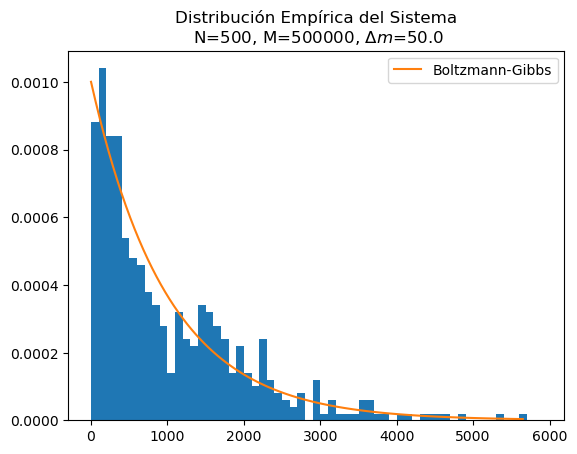
\includegraphics[width=0.4\linewidth]{img/ejSimulacion.png}
\caption{}
\end{figure}



\newpage
\begin{thebibliography}{}
    \bibitem{Yakovenko} A. Dr\u{a}gulescu, V.M. Yakovenko. (2000). Statistical mechanics of money.
    \bibitem{Scalas} Bertram Düring, Nicos Georgiou and Enrico Scalas. (2016) A stylized model for wealth distribution. 
    \bibitem{Wannier} G.H. Wannier. (1987) Statistical Physics.
\end{thebibliography}

\end{document}

%%%%%%%%%%%%%%%%%%%%%%%%%%%%%%%%%%%%%%%%%%%%%%%%%%%%%%%%%%%%%%%%%%%%%%%%%%%%%%%%%%%%%%%%%%%%
%%%%%%%%%%%%%%%%%%%%%%%%%%%%%%%%%%%%%%%%%%%%%%%%%%%%%%%%%%%%%%%%%%%%%%%%%%%%%%%%%%%%%%%%%%%%


